\section{Regression}

Der zweite Teil der Arbeit beschäftigt sich mit der Regression.
Während die zuvor behandelte Korrelation nur die Stärke eines Zusammenhangs zwischen Merkmalen feststellt, ist es mittels der Regression möglich, genauere Informationen zu erhalten.
Die Regression versucht dazu, die Werte eines abhängigen Merkmals (Regressand) mittels einer Funktion von den Werten eines oder mehreren unabhängigen Merkmalen (Regressoren) abzuleiten.

Die \naglib bietet dazu zahlreiche Funktionen, von verschiedenen Regressionsarten bis hin zu Hilfen für die Bewertung und Validierung von Regressionsmodellen.
Diese Arbeit wird sich dabei auf zwei verschiedene Regressionsmodelle konzentrieren:
Die einfache lineare Regression und die multiple lineare Regression.
Für beide werden die mathematischen Grundlagen behandelt, sowie die Berechnungen durch die \naglib erklärt. 
Außerdem wird für beide Regressionsarten anhand des Beispiels des Münchener Mietspiegels die Anwendung demonstriert.

In der nächsten Sektion wird zunächst die einfache Regression vorgestellt, welche sich mit der Abhängigkeit eines Merkmals von einem Anderen beschäftigt.
Für die theoretischen Grundlagen wurden \cite{Cramer2007} und \cite{Fahrmeir2010} gemeinsam mit der Einführ"-ung zur \naglib (\cite{nag:intro}) verwendet.

\subsection{Einfache Regression}
\label{sec:sim_reg}

Bei Anwendung der einfachen Regression existiert immer nur ein Regressor, für welchen der Einfluss auf ein anderes Merkmal untersucht werden soll.
Dennoch reicht diese einfache Form schon für viele Anwendungen aus, zum Beispiel wenn wir die Höhe der Mietpreise ($M$) in Abhängigkeit von der Anzahl der Räume ($R$) betrachten (vgl. Abschnitt \ref{sec:beispiel}).
In diesem Falle ist der Mietpreis der Regressand und die Raumanzahl ist der Regressor, zudem ist in Abbildung \ref{fig:nm_rooms_distribution} zu erkennen, dass die Nettomiete metrisch und die Raumanzahl verhältnisskaliert ist.
\begin{figure}[t]
  \centering
  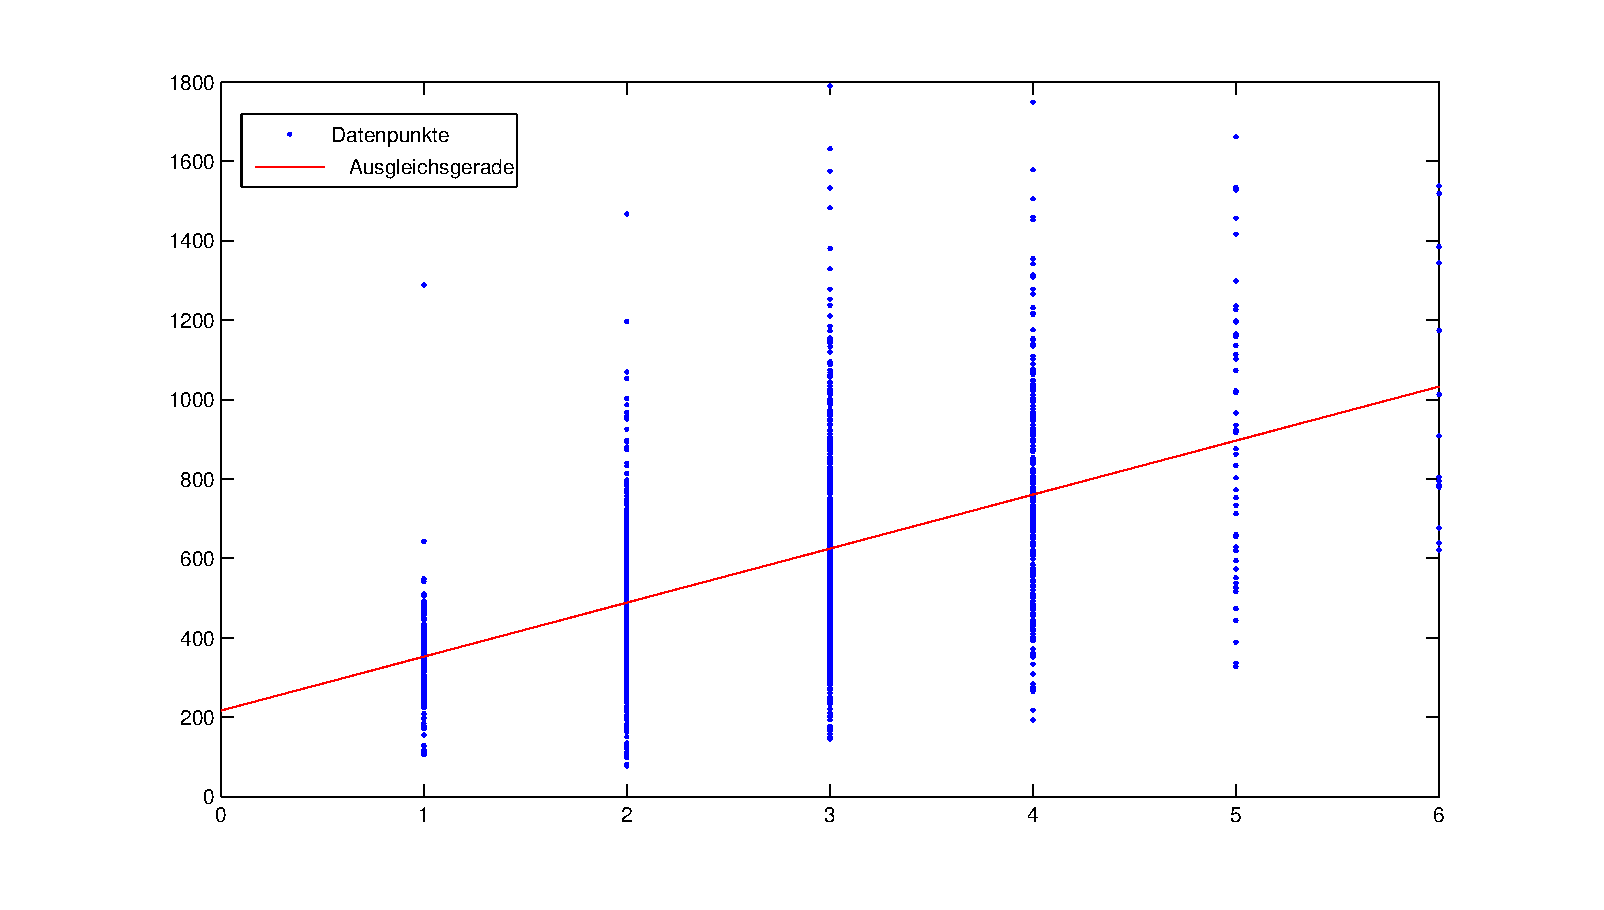
\includegraphics[width=0.8\textwidth]{figures/nm_rooms_distribution}
  \caption{Verteilung der Nettomieten in Abhängigkeit von der Raumanzahl mit der berechneten Ausgleichsgeraden. Datensatz: Münchener Mietspiegel 2003 \cite{Fahrmeir2011}.}
  \label{fig:nm_rooms_distribution}
\end{figure}
Ziel der Regression ist es nun, den Mietpreis als Funktion der Raumanzahl darzustellen:
\begin{equation*}
 M = f(R) + \epsilon ~.
\end{equation*}
Dabei ist $f$ eine beliebige Funktion und $\epsilon$ ein Fehlerterm.
Dieser wird benötigt, da die den Merkmalen zugehörigen Datensätze $(m_1, \dots, m_n)$, bzw. $(r_1, \dots, r_n)$ nie \textit{genau} auf der Regressionsgeraden liegen, sondern durch Messfehler oder nicht berücksichtigte Abhängigkeiten abweichen.
Der Erwartungswert für diese Fehler ist immer $0$. 
Um auch für kleinere Stichproben Aussagen über die Verteilung der Schätzer machen zu können, wird meinst zusätzlich eine Normalverteilung angenommen \cite[S. 479]{Fahrmeir2010}:
\begin{equation*}
  E(\epsilon_i) = 0 \text{ und } \epsilon_i \sim N(0,\sigma^2), i = 1, \dots, n ~.
\end{equation*}
Diese Arbeit konzentriert sich nur auf lineare Funktionen $f$, aber in Abschnitt \ref{sec:mult_reg} wird gezeigt, wie auch ein logarithmischer Zusammenhang zwischen Regressand und Regressor miteinbezogen werden kann.
Hier ist aber ein linearer Zusammenhang naheliegend, daher wählen wir auch einen einfachen linearen Ansatz:
\begin{equation*}
  M = \alpha + \beta R + \epsilon ~.
\end{equation*}
Dieser Ansatz lässt sich natürlich auf beliebige Merkmale übertragen.
Um nun die Ausgleichsgerade wie in Abbildung \ref{fig:nm_rooms_distribution} zu erhalten, ist es nötig die Parameter $\alpha$ und $\beta$ so zu schätzen, dass der quadratische Fehler minimal wird.
Dieses Verfahren wird  \textit{Methode der kleinsten Quadrate} (KQ-Methode) genannt.
Formal sieht der Ansatz wie folgt aus:
\begin{equation*}
  \sum\limits_{i=1}^{n} \epsilon^2 = \sum\limits_{i=1}^{n} (m_i - \alpha - \beta r_i)^2 \rightarrow \min\limits_{\alpha, \beta} ~.
\end{equation*}
Die minimierenden Werte werden mit $\hat\alpha$ und $\hat\beta$ notiert und als \textit{Kleinste-Quadrate-Schätzer} bezeichnet.
Für unseren linearen Ansatz können beide Schätzer relativ einfach berechnet werden.
Der Regressionskoeffizient $\hat\beta$ ist allgemein für zwei Merkmale $X$ und $Y$ gegeben durch
\begin{equation*}
  \hat\beta = \frac{\tilde s_{XY}}{\tilde{s}^2_X} = \frac{\sum\limits_{i=1}^{n} y_i x_i - n \bar y \bar x}{\sum\limits_{i=1}^{n} x_i^2 - n \bar{x}^2} ~.
\end{equation*}
wobei $\tilde{s}^2_X$ die Varianz von $X$ und $\tilde s_{XY}$ die Kovarianz von $X$ und $Y$ bezeichnet. 
Wenn der Koeffizient bekannt ist, kann er in dir folgende Gleichung eingesetzt werden um die Konstante $\alpha$ zu erhalten:
\begin{equation*}
  \alpha = \bar y - \hat\beta \bar x ~.
\end{equation*}
Die Beweise für beide Rechnungen wurden hier aus Platzgründen ausgelassen, sind aber in \citet[S. 155]{Fahrmeir2010} zu finden.
% TODO: Muss der Durchschnitt hier erklärt werden?

Mithilfe dieser Methode erhalten wir nun die Schätzer für unser Beispiel.
Durch einfaches Einsetzen der Daten erhalten wir folgendes Ergebnis (Alle Zahlen wurden auf eine Stelle hinter dem Komma gerundet):
\begin{equation*}
  \hat\beta = \frac{\sum\limits_{i=1}^{n} m_i r_i - n \bar m \bar r}{\sum\limits_{i=1}^{n} r_i^2 - n \bar{r}^2}
  = \frac{3309500 - 2053 * 570.1 * 2.6}{15833 - 2053 * 2.6^2}
  \approx 136
\end{equation*}
\begin{equation*}
  \hat\alpha = \bar m - \hat\beta \bar r 
  = 570.1 - 136 * 2.6 
  \approx 216.8 ~.
\end{equation*}
Somit hat die Ausgleichsgerade in Abbildung \ref{fig:nm_rooms_distribution} die Gleichung $\hat m = 216.8 + 136 r$
Wir schreiben hier $\hat m$, da die Regressionsgerade eine Schätzung für die Nettomiete ist.

Die anfängliche Vermutung eines linearen Zusammenhangs zwischen der Anzahl der Zimmer und der Nettomiete ist damit bestätigt.
Man kann das Ergebnis weiterhin so interpretieren, dass es für jede Wohnung eine Grundmiete in Höhe von \EUR{216,80} gibt, die dann pro Zimmer um \EUR{136} erhöht wird.
Diese Interpretation ist allerdings in diesem Fall nicht unbedingt zielführend, da man schon mit bloßem Auge erkennen kann, dass die Residuen (Abweichungen der einzelnen Datenpunkte von der Ausgleichsgeraden) groß sind.
Daher wird die Annahme, wenn auch grundsätzlich richtig, wohl nur auf wenige Wohnungen zutreffen.
\\

Die Berechnung in der Funktion nag\_simple\_linear\_regression der \naglib erfolgt grundsätzlich wie oben beschrieben, allerdings mit einer Ausnahme: Es ist zusätzlich möglich die einzelnen Datenpunkte zu gewichten.
Dies führt dazu dass bei der Methode der kleinsten Quadrate auch die Fehler gewichtet eingehen, daher ist der Ansatz zur Minimierung dann $\sum\limits_{i=1}^{n}w_i\epsilon_i \rightarrow min$, wobei $w_i$ die Gewichtungen für die einzelnen Datenpunkte sind.
Für eine vollständige Beschreibung der Berechnungen mit Gewichtung sei der Leser auf \cite{nag:simple_regression} verwiesen.

\subsubsection{Methodenaufruf}
\label{sec:sim_reg_anwendung}

Nach der Beschreibung der Berechnung der einfachen linearen Regression wollen wir nun auf die Anwendung mittels der Funktion nag\_simple\_linear\_regression eingehen.
Die Funktionsdeklaration ist in Listing \ref{lst:nag_simple_linear} zu sehen.
\begin{figure}[t]
  \begin{lstlisting}[caption={Deklaration der Methode \glqq nag\_simple\_linear\_regression\grqq, mit der eine einfache lineare Regression berechnet werden kann.}\label{lst:nag_simple_linear}, captionpos=b]
    void nag_simple_linear_regression (Nag_SumSquare mean, 
    Integer n, const double x[], const double y[], 
    const double wt[], double *a, double *b, double *a_serr, 
    double *b_serr, double *rsq, double *rss, double *df,
    NagError *fail)
  \end{lstlisting} 
\end{figure}
Es existieren insgesamt 13 Parameter, von denen die ersten Fünf Eingabe- und die Restlichen Ausgabeparameter sind.

Die wichtigsten Eingabeparameter sind die beobachteten Werte für das unabhängige(\lstinline{x[]}) und das abhängige(\lstinline{y[]}) Merkmal.
Für den Parameter \lstinline{n} muss nur die Anzahl der Beobachtungen angegeben und für \lstinline{wt[]} kann ein Array mit Gewichtungen für eingetragen werden.   
Falls keine Gewichtung gewünscht ist genügt es einen Null-Zeiger (zB. \lstinline{(double *) 0}) anzugeben.
Zuletzt existiert noch \lstinline{mean}.
Falls hier der Wert 'Nag\_AboutZero' angegeben wird, wird die Konstante $\alpha$ nicht in den Regressionsansatz miteinbezogen, d.h. die Regressionsgerade geht in jedem Fall durch den Ursprung.
Für die normale Berechnung kann 'Nag\_AboutMean' angegeben werden.

Die Ergebnisse der Regression $\hat\alpha$ und $\hat\beta$ sind nach Ausführung der Methode über die Zeiger \lstinline{*a} und \lstinline{*b} erreichbar.
Zudem werden auch einige Informationen zurückgegeben, die helfen die Güte des Regressionsansatzes zu überprüfen.
Da sind zunächst die Standartfehler \lstinline{*a_serr} und \lstinline{*b_serr}, die einen Hinweis darauf geben, wie genau die Koeffizienten geschätzt werden konnten.
Einen Hinweis auf die Güte des Regressionsmodells gibt das Bestimmtheitsmaß $R^2$ in \lstinline{*rsq}.
Es sagt aus, ein wie großer Anteil einer Variation des abhängigen Merkmals durch das unabhängige Merkmal erklärt wird.
Definiert ist es als Quadrat der Korrelation $R^2 = r_{XY}^2$ und nimmt daher Werte zwischen 0 und 1 an.
Ist der Wert niedrig, deutet dies auf ein schlechtes Regressionsmodell hin, da der Wert der abhängigen Variable dann stark von anderen, nicht beachteten, Einflüssen abhängig ist.
Zusätzlich wird noch die Summe der Fehlerquadrate (der minimierte Wert) in \lstinline{*rss} geschrieben.
Falls diese Summe sehr groß ist, weist das darauf hin, dass die Regressionsfunktion eine zu niedrige Komplexität haben könnte, um den Zusammenhang zwischen Regressor und Regressand hinreichend abzubilden.
Zuletzt gibt die Funktion über \lstinline{*fail} einen Fehler vom Typ \lstinline{NagError} aus, falls die Eingabeparameter falsch gesetzt wurde, oder das SVD Verfahren nicht konvergiert.

% TODO: Erwähnen, dass Beispielaufruf in Beispielprogramm verfügbar ist.

\begin{comment}
\begin{itemize}
 \item Nichtlineare Regression
 \begin{itemize}
  \item Für Sättigungskurven und Wachstumsverläufe
  \item Mögliche Funktionen: exp, $x^2$, sin
  \item Berechnung durch kleinste Quadrate Methode mittels Transformation möglich
 \end{itemize}

 \item Beispiel: Regression der Nettomiete nach Wohnfläche
 \begin{itemize}
  \item Streudiagramm zeigt steigende Abweichung $\Rightarrow$ Multiple Regression nötig!
 \end{itemize}
\end{itemize}

\subsubsection{Beispiel}


\end{comment}

\subsection{Multiple Lineare Regression}
\label{sec:mult_reg}

% TODO: Referenzen!

Im letzten Abschnitt haben wir behandelt, wie man mittels einfacher Regression die Werte eines abhängigen Merkmals auf Grundlage der Werte eines unabhängigen Merkmals schätzen kann.
Allerdings stößt die einfache Regression an Grenzen, wenn der Regressand von vielen Merkmalen beeinflusst wird, wobei die einzelnen Korrelationen an sich schwach sind.
Weiterhin bleiben offene Fragen: 
Wie verändert sich die Verteilung der Nettomieten zur Wohnfläche mit steigendem Baujahr?
Und wie groß ist der Einfluß von guter bzw. bester Wohnlage auf den Wohnungspreis? 
Diese können mit der multiplen linearen Regression gelöst werden, welche nun vorgestellt wird.

% Für die Berechnung über Matrizen wird \cite{Fahrmeir1984} für die theoretischen Grundlagen verwendet.
Die multiple Regression ist zunächst einmal eine Erweiterung der einfachen Regression auf eine beliebige Anzahl von Regressoren.
Dementsprechend wird auch das Regressionsmodell selbst auf $p$ unabhängige Merkmale erweitert:
\begin{equation*}
  Y_i = \beta_0 + \beta_1 x_{i1} + \dots + \beta_p x_{ip} + \epsilon_i, \quad i = 1, \dots, n ~.
\end{equation*}
Die Notation ist wie folgt:
Das abhängige Merkmal $Y$ ist in den Zufallsvariablen $Y_i, \dots, Y_n$ modeliert und $x_{1j}, \dots, x_{nj}$ sind jeweils die beobachteten Werte für die $j$ verschiedenen Regressoren.
Außerdem sind die Fehlerterme $\epsilon_1, \dots, \epsilon_j$ genauso modeliert wie in Sektion \ref{sec:sim_reg} und $\beta_0$ bis $\beta_n$ bezeichnen die Regressionskoeffizienten.
$\beta_0$ nimmt dabei die Rolle des konstanten Terms ein, den zuvor $\alpha$ innehatte.

Die Idee zur Berechnung der Koeffizienten ist die Selbe wie zuvor:
Wieder wird die kleinste Quadrate Methode verwendet und den quadratischen Fehler zu minimieren:
\begin{equation*}
  \label{eq:kq_mul}
  \sum\limits_{i=1}^{n} (Y_i - \beta_0 -\beta_1 x_1 - \dots - \beta_p x_{ip})^2 \rightarrow \min\limits_{\beta_0,\beta_1,\dots,\beta_n} ~.
\end{equation*}
Damit dieses Minimierungsproblem eine eindeutige Lösung $\hat\beta_0, \hat\beta_1, \dots, \hat\beta_p$ hat, müssen nach \citep[S.496]{Fahrmeir2010} die beiden folgenden Voraussetzungen erfüllt sein:
\begin{enumerate}
  \item Es müssen mindestens so viele Beobachtungen vorliegen, wie es Variablen im Regressionsansatz gibt. 
    Für gute Schätzungen sollte die Anzahl der Beobachtungen sogar deutlich größer sein.
  \item Die Merkmale müssen voneinander unabhängig sein, d.h. es darf nicht möglich sein eine Regressionsvariable als Linearkombination der anderen Variablen zu schreiben: $X_j \neq \sum\limits_{k\neq j} a_k X_k + b,~ \forall a_k, b$ muss gelten!
    Ist dies nicht der Fall ist mindestens eine der Variablen überflüssig, da mehrere den gleichen Anteil der Varianz des Regressanden erklären.  
\end{enumerate}

Auch wenn das Modell der multiplen linearen Regression nicht bedeutend komplexer als das der einfachen linearen Regression erscheint, so ist die Berechnung doch ungleich schwieriger.
So ist es jetzt nicht mehr möglich einfache direkte Formeln für die Berechnung der Regressionskoeffizienten anzugeben.
Stattdessen erfolgt die Berechnung nun mit Hilfe von Matrizen und Vektoren.
Als nächstes wollen wir zeigen wie genau die multiple Regression von der \naglib berechnet wird.
Auf die Demonstration der Berechnung anhand der Beispieldaten wird dabei verzichtet, allerdings wird das Ergebnis einer Regression in Sektion \ref{sec:reg_mul_ergebnis} vorgestellt und interpretiert.

\subsubsection{NAG Algorithmus}

In der NAG-Bibliothek wird die multiple Regression hauptsächlich durch die Funktion nag\_regsn\_mult\_linear zur Verfügung gestellt.
% TODO: KQ_Methode vorher definieren
Da die Berechnung wie bereits erwähnt mit Hilfe von Matrizen erfolgt, können wir den Minimierungsan"-satz der KQ-Methode wie folgt anpassen:
\begin{equation*}
  \label{eq:minimization}
  \sum\limits^{N}_{n=1} \epsilon^2_n = \epsilon^T \epsilon = (y - X \beta)^T (y - X \beta) \rightarrow \min\limits_{\beta} ~.
\end{equation*}
$\epsilon$ ist dabei der Vektor, der alle $\epsilon_i$ enthält und $X$ ist eine $n \times p$ Matrix mit den beobachteten Werten für alle Regressoren.
Außerdem sind $y$ und $\beta$ Vektoren, die beobachteten Werten für den Regressanden und die Koeffizienten beinhalten. 
Der erste Schritt ist dabei nur ein formales Umschreiben des KQ-Ansatzes durch Vektoren.
Anschließend werden die Fehlervektoren, durch ihre Definition, die Abweichung der berechneten Werte ($X\beta$) von den tatsächlichen Werten ($y$), ersetzt.
Da der Wurzel-Operator keinen Einfluß auf den Wert des Minimums hat, können wir die Forderung wie folgt umformulieren:
\begin{equation*}
  \label{eq:minimization_general}
  \Vert X\beta - y \Vert_2 \rightarrow \min\limits_{\beta} ~.
\end{equation*}
Um dieses Minimum zu erhalten, wird in nag\_regsn\_mult\_linear die QR-Zerlegung der Matrix $X$ berechnet.

Für die QR-Zerlegung gilt $X = QR$, wobei $Q$ eine orthogonale Matrix und $R$ eine obere rechte Dreiecksmatrix ist.
Die drei am meisten verbreiteten Verfahren zur Berechnung einer QR-Zerlegung sind folgende \citep[S. 211ff]{Golub1989}: Householder Transformationen, Givens Rotationen und das modifizierte Gram-Schmidt Verfahren.
Es ist nicht bekannt welches dieser Verfahren von der \naglib verwendet wird, allerdings sind nach \cite{Golub1989} sowohl das modifizierte Gram-Schmidt Verfahren (S.227), als auch die Givens Rotationen (S.228) langsamer als die Householder Transformationen, wenn es um die Lösung von Ausgleichsproblemen geht.
Für unsere Berechnung können wir uns nun einige Eigenschaften der Matrizen $Q$ und $R$ zunutze machen und den zu minimierenden Term erneut umschreiben:
\begin{equation*}
  \label{eq:orthogonal_transformation}
  \Vert X\beta - y \Vert_2 = \Vert Q^T X \beta - Q^T y \Vert_2 = \Vert R_1 \beta - c \Vert_2 + \Vert d \Vert_2 ~.
\end{equation*}
Im ersten Schritt kommt uns zugute, dass die 2-Norm bei orthogonaler Transformation den Wert erhält.
Daher können wir den Term mit $Q^T$ multiplizieren (die Orthogonalität wird beim Transponieren erhalten).
Eine weitere praktische Eigenschaft von orthogonalen Matrizen ist es, dass die transponierte Matrix zugleich die Inverse ist.
Daher folgt aus $X = QR_1$ sofort $Q^T X = R_1$.
Der Vektor $c$ ist einfach definiert als das Ergebnis der Operation $Q^T y$.
Die letzte Umformung gibt auch direkt den nach der Minimierung verbleibenden Restfehler in $\|d\|_2$ an, weswegen es nun möglich ist $\|R_1\beta - c\|_2 = 0$ zu verlangen.

Um nun die Werte für die Koeffizienten zu erhalten, muss das folgende Gleichungssystem gelöst werden:
\begin{equation*}
  R\hat\beta = c_1 ~.
\end{equation*}
Dabei gilt $R_1 = \begin{bmatrix} R \\ 0\end{bmatrix}$ ($R$ enthält nur die ersten $p$ Zeilen aus $R_1$) und $c_1$ ist ein Vektor mit den ersten $p$ Einträgen aus $c$. 
Da $R$ eine obere rechte Dreiecksmatrix ist, ist dies durch Rückwärtseinsetzen möglich.
Dies führt allerdings nur zu einem eindeutigen Ergebnis, falls $R$ vollen Rang hat.
Da diese Forderung aber äquivalent dazu ist, dass $X$ einen vollen Rang hat \citep[S. 225]{Golub1989}, können wir in unserem Anwendungsfall davon ausgehen, dass dies fast immer zutrifft, da die Zahl der Beobachtungen ohnehin immer größer sein sollte als die Zahl der einbezogenen Merkmale (und die Beobachtungen normalerweise verschieden sind).
Falls der Rang von $R$ dennoch nicht voll sein sollte, wird die Singulärwertzerlegung (SVD-Verfahren) angewandt um ein Ergebnis zu finden. 
Diese wird hier nicht vorgestellt, weitere Informationen können aber in \cite{nag:g02dac} und \citep[S. 239f]{Golub1989} gefunden werden.

\begin{comment}
\subsubsection{Singulärwertzerlegung}
Wie zuvor bereits erwähnt, wird die Singulärwertzerlegung in nag\_regsn\_mult\_linear nur angewandt, wenn der Rang der Matrix $R$ und damit auch der Rang von $X$ nicht voll ist.
Da die Zahl der Beobachtungen aber ohnehin immer größer sein sollte als die Zahl der einbezogenen Merkmale (und die Beobachtungen normalerweise verschieden sind), sollte dieser Fall bei normaler nicht allzu oft eintreten, weswegen wir die Singulärwertzerlegung hier nur kurz behandeln.  
\end{comment}

\subsubsection{Anwendung}
\label{sec:reg_mul_ergebnis}

Nun wollen wir zeigen, wie wir die multiple Regression am Beispiel des Mietspiegeldatensatzes nutzen können.
Um die Fragen vom Anfang dieses Abschnitts zu beantworten, wählen wir einen Regressionsansatz mit der Nettomiete ($NM$) als Regressanden und den unabhängigen Merkmalen Wohnfläche($W$), gute Wohnlage($gL$) und Baujahr($Bj$) als Regressoren.
In diesem Fall lohnt es sich einen Blick auf die Verteilung der Nettomieten zu werfen, bevor der Regressionsansatz festgelegt wird.
Diese Verteilung ist in Abbildung \ref{fig:nm_wfl_distributions:normal} in Abhängigkeit von der Wohnfläche zu sehen.
\begin{figure}[t]
  \centering
  \begin{narrow}{-0.2\textwidth}{0.2\textwidth}
    \subfloat[][Normale Skala]{
      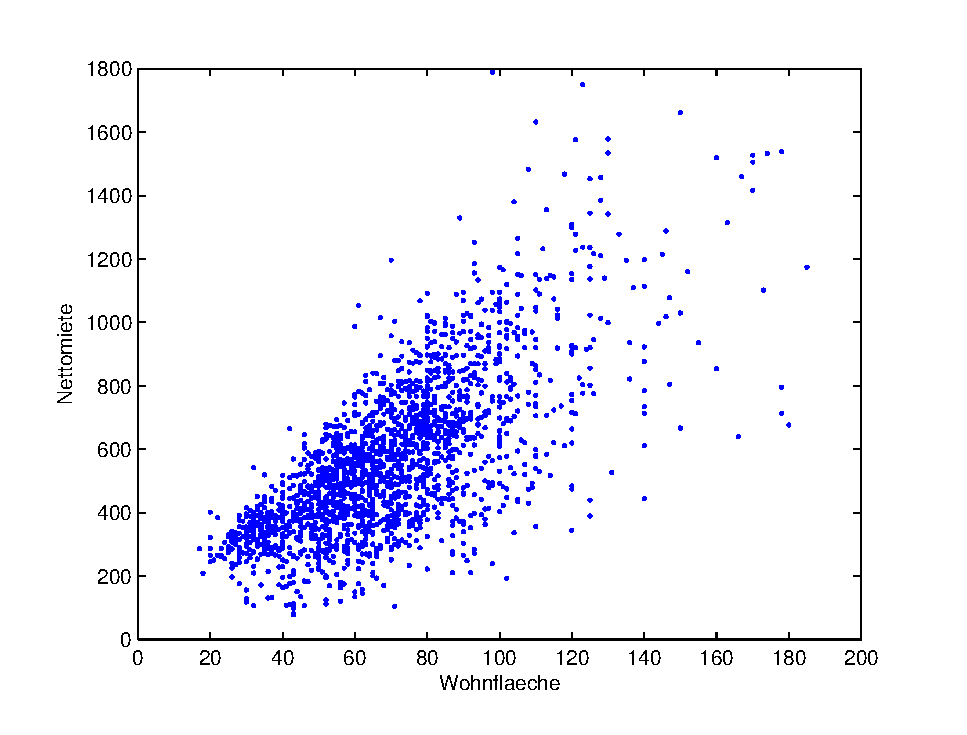
\includegraphics[width=0.7\textwidth]{figures/nm_wfl_distribution}
      \label{fig:nm_wfl_distributions:normal}
    }
    \subfloat[][Logarithmische Skala]{
      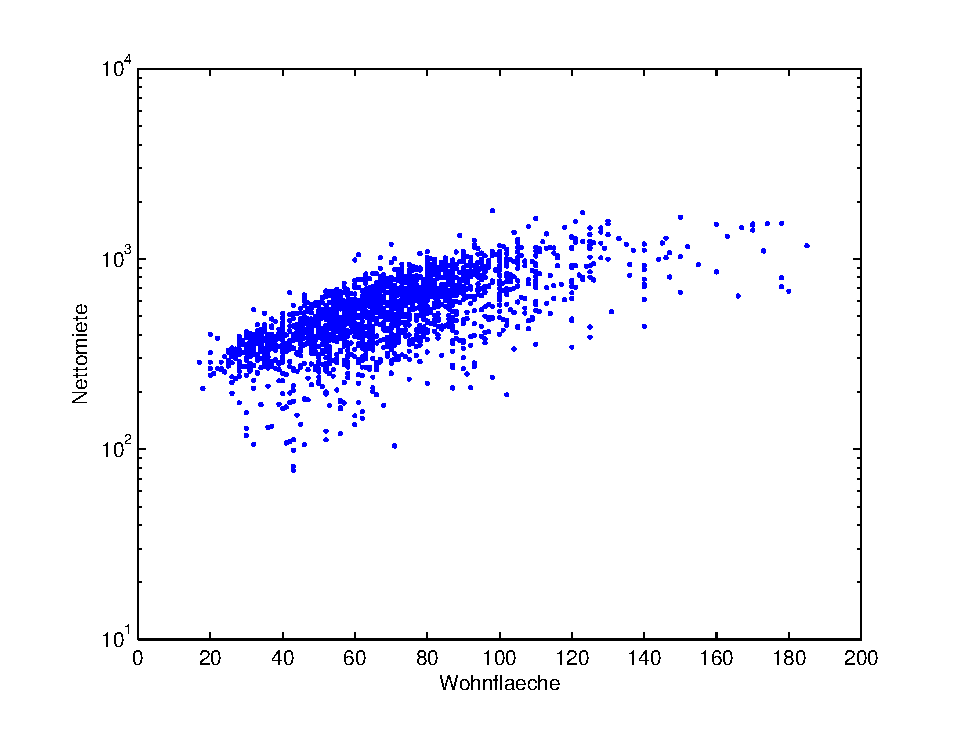
\includegraphics[width=0.7\textwidth]{figures/nm_wfl_distribution_log}
      \label{fig:nm_wfl_distributions:log}
    }
   
  \end{narrow}
  \caption{Die Verteilung der Nettomieten in Abhängigkeit von der Wohnfläche im Mietspiegel Datensatz.}
  \label{fig:nm_wfl_distributions}
\end{figure}
Es ist erkennbar, dass die Größe der Fehler mit steigender Wohnfläche zunimmt, was die Güte des Ergebnisses vermindert.
Eine bessere Verteilung ist mit einer logarithmischen Skala erkennbar (vgl. Abb. \ref{fig:nm_wfl_distributions:log}), weswegen wir $log(NM)$ anstelle von $NM$ als Zielvariable wählen:
\begin{equation*}
 log(NM) = \beta_0 + \beta_1 W + \beta_2 Bj + \beta_3 gL + \epsilon ~.
\end{equation*}

Unter Benutzung des zuvor vorgestellten Algorithmus erhalten wir folgenden Vektor mit den Regressionskoeffizienten:
\begin{equation*}
  \beta = \begin{pmatrix} \beta_0 \\ \beta_1 \\ \beta_2 \\ \beta_3 \end{pmatrix} = \begin{pmatrix} -2.83 \\ 0.01 \\ 0.004 \\ 0.11 \end{pmatrix}
\end{equation*}
Wenn diese Werte jetzt wieder in den Regressionansatz eingesetzt werden, erhalten wir das Ergebnis:
\begin{eqnarray*}
  \log(NM) & = & -2.83 + 0.01 W + 0.004 Bj + 0.11 gL + \epsilon\\
  \Rightarrow NM & = & \exp(-2.83) \exp(0.01 W) \exp(0.004 Bj) \exp(0.11 gL) ~.
\end{eqnarray*}
In der zweiten Zeile wurde der Regressionsansatz dabei wieder rücktransformiert, damit wir eine Aussage über die Nettomiete erhalten und nicht über ihren Logarithmus.

Da das Merkmal \glqq gute Wohnlage\grqq~ binär ist, können wir nun noch die Basismiete und den Aufpreis für eine Wohnung in guter Wohnlage bestimmen: $NM = NM_B \alpha$.
Die Basismiete $NM_B$ ergibt sich, wenn $gL$ auf 0 gesetzt wird:
\begin{equation*}
  NM_B = 0.059 \cdot \exp(0.012 W) \exp(0.004 Bj) ~.
\end{equation*}
Dieses Verhältnis zwischen Nettobasismiete, Wohnfläche und Baujahr ist in Abbildung \ref{fig:3d_result} geplottet.
\begin{figure}[t]
  \centering
  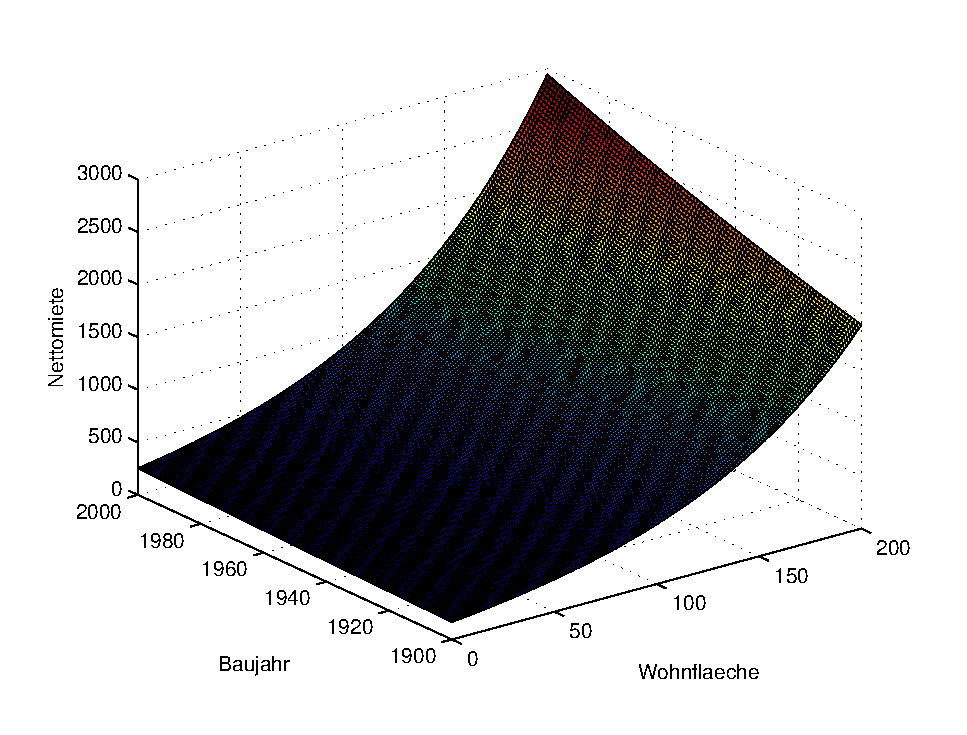
\includegraphics[width=10cm]{figures/nm_wfl_bj_log_approach}
  \caption{Das Ergebnis der Regression der Nettomiete mit den Regressanden Wohnfläche und Baujahr.}
  \label{fig:3d_result}
\end{figure}
Man kann erkennen, dass die Nettomiete sowohl mit zunehmendem Baujahr als auch mit zunehmender Wohnfläche ansteigt, was auch den Erwartungen entspricht.
Zusätzlich dazu kann man aber noch sehen, dass die Miete im Verhältnis zur Wohnfläche mit neuerem Baujahr immer schneller wächst, ein Ergebnis, das mit der einfachen Regression nicht hätte erreicht werden können.

Der Aufschlag für gute Wohnlage geht dann als Faktor in die Berechnung ein: $\alpha = exp(0.105) = 1.111$.
Für eine Wohnung in guter Wohnlage muss also mit einem Aufschlag von $11.1 \%$ auf die Basismiete gerechnet werden.


\subsubsection{Methodenaufruf}

Bei Benutzung der \naglib kann die multiple Regression durch die Funktion nag\_regsn\_mult\_linear berechnet werden.
Die Deklaration dieser Methode wird in Listing \ref{lst:nag_multiple_linear} gezeigt.
\begin{figure}[t]
\begin{lstlisting}[caption={Deklaration der Methode nag\_regsn\_mult\_linear, welche eine multiple lineare Regression ausführt.}\label{lst:nag_multiple_linear},captionpos=b]
void nag_regsn_mult_linear (Nag_IncludeMean mean, Integer n, 
    const double x[], Integer tdx, Integer m, 
    const Integer sx[], Integer ip, const double y[], 
    const double wt[], double *rss, double *df, double b[], 
    double se[], double cov[], double res[], double h[], 
    double q[], Integer tdq, Nag_Boolean *svd, Integer *rank, 
    double p[], double tol, double com_ar[], NagError *fail)
\end{lstlisting}
\end{figure}

Da die Methode sehr viele Parameter (24) hat, werden wir uns hier auf die Interessantesten beschränken.
Einige Parameter sind zudem äquivalent zu Parametern der Funktion nag\_simple\_linear\_regression, welche bereits in Sektion \ref{sec:sim_reg_anwendung} behandelt wurden und können auch genau so verwendet werden.
Diese sind: \lstinline{mean}, \lstinline{n}, \lstinline{x[]}, \lstinline{y[]}, \lstinline{wt[]}, \lstinline{*rss} und \lstinline{*fail}.
Für \lstinline{x[]} muss in diesem Fall verständlicherweise eine Matrix statt eines Vektors angegeben werden und die zulässigen Werte für \lstinline{mean} sind Nag\_MeanInclude (konstanten Term miteinbeziehen) und Nag\_MeanZero (kein konstanter Term).

Zu den genannten Parametern kommen weitere Eingabeparameter hinzu, mit denen die Regressoren aus den Merkmalen im Datensatz ausgewählt werden können.
Die Gesamtzahl an unabhängigen Variablen im Datensatz wird in \lstinline{m} gesetzt.
Im Vektor \lstinline{sx[]} der Länge $m$ wird dann für alle Regressoren ein Wert $>0$ eingetragen, alle anderen Felder erhalten eine Null.
Die Anzahl der Regressoren muss zusätzlich in \lstinline{ip} gegeben werden.
Für \lstinline{tol} muss zudem ein Toleranzwert angegeben werden, der bestimmt, wie groß der Unterschied zwischen zwei Zahlen sein darf, damit diese im Algorithmus noch als gleich groß behandelt werden. 
Das hat vor allem Auswirkungen auf den Rang der unabhängigen Variablen und beeinflusst damit, ob das SVD-Verfahren zum Einsatz kommt (Falls \lstinline{tol=0} verwendet wird ist dies nie der Fall).

Die Ausgabeparameter sind großteils von denen der einfachen Regressionsfunktion verschieden.
Am wichtigsten ist \lstinline{b[]}, welcher die berechneten Koeffizienten $\beta_0, \beta_1, \dots$ enthält.
Wie zuvor werden auch hier die zugehörigen Standartfehler in \lstinline{se[]} zurückgegeben.
Dazu kommen nun noch die Residuen für jede Beobachtung im Datensatz in \lstinline{res[]}, welche es einfach machen Ausreißer zu identifizieren.
Nach der Regression stehen außerdem Informationen zu den Verhältnissen der Regressoren untereinander in Form einer Kovarianzmatrix (\lstinline{cov}) zur Verfügung.
Diese enthält die Varianzen der Merkmale auf der Diagonalen und zudem alle möglich Kombinationen an Kovarianzen, was zum Beispiel ein schnelle Berechnung der Pearson-Korrelation ermöglicht (siehe auch Sektion \ref{sec:corr_per}).
Zuletzt geben \lstinline{*rank} und \lstinline{*svd} noch den Rang der Regressoren an und ob bei der Berechnung die Singulärwertzerlegung benutzt wurde.
\\

Zusätzlich zu nag\_regsn\_mult\_linear stellt die \naglib einige andere Funktionen zu Verfügung, die es ermöglichen das Regressionsmodell zu ändern, ohne die gesamte Regression erneut zu berechnen.
Diese Funktionen benötigen neben anderen Argumenten die QR-Zerlegung (welche von der Hauptfunktion als Zwischenergebnis in \lstinline{q[]} ausgegeben wird), die zugehörigen Informationen (\lstinline{p[]}) und die Beobachtungsmatrix $X$ und berechnen daraus aktualisierte Werte für die obere rechte Dreiecksmatrix $R$ und den Vektor $c$.
Im Gegensatz zu einer erneuten Berechnung mittels nag\_regsn\_mult\_linear hat dies den Vorteil, dass durch die Benutzung eines bereits bekannten Zwischenergebnisses Rechenzeit eingespart werden kann.
So kann der Benutzer beispielsweise mit nag\_regsn\_mult\_linear\_addrem\_obs neue Beobachtungen zum Modell hinzufügen oder sie entfernen.
Mit den Methoden nag\_regsn\_mult\_linear\_delete\_var und nag\_regsn\_mult\_linear\_add\_var werden aus dem Modell herausgenommen bzw. hinzugefügt, wobei die Beobachtungen im letzteren Fall schon in $X$ enthalten sein sollten.
Zusätzlich dazu ist es auch noch möglich die abhängige Variable zu tauschen (nag\_regsn\_mult\_linear\_newyvar).

Nach Anwendung dieser Funktionen können die neuen Regressionskoeffizienten $\beta_0, \beta_1, \dots$ durch einen Aufruf von nag\_regsn\_mult\_linear\_upd\_model unter Angabe von $R$ und $c$ erhalten werden.
Die einzelnen Funktionen werden in dieser Arbeit nicht einzeln diskutiert, weitere Informationen sind aber unter \citep{nag:contents} verfügbar.






%\subsection{Analyse}

%TODO:Überarbeiten oder herausnehmen!
%Zusätzlich zu der Berechnung der verschieden Regressionsmodelle bietet die {\it NAG C Library} auch Funktionen zur Auswahl des Regressionsmodells und zur Modellvalidierung.

%Für die Auswahl des Modells sollen in der Arbeit zwei Metriken behandelt werden: Die Residualstreuung und das Bestimmtheitsmaß $\mathcal{R}^2$.
%Beide können uns eine Idee davon geben, wie gut die unabhängigen Variablen die Werte der abhängigen Variablen erklären können.
%Die Residualstreuung gibt die Verteilung der Differenzen zwischen der angenäherten Funktion und den wirklichen Daten an.
%Sollte sie unregelmäßig sein (wenn die Residuen beispielsweise mit einer Variablen anwachsen) ist dies ein starkes Indiz dafür, dass ein zu simples Modell gewählt wurde. 
%Das Bestimmtheitsmaß gibt dagegen an, wie gut abhängige Variable durch die Regression erklärt werden kann.
%Berechnet werden kann es auch durch eine Quadrierung des Bravais-Pearson Korrelationskoeffizienten, was den starken Zusammenhang von Korrelation und Regressionsanalyse zeigt.

%Für die Modellvalidierung stehen verschiedene Werkzeuge zur Verfügung, welche bei der Bewertung der Güte der Regression und deren Verbesserung genutzt werden können.
%In diese Kategorie fallen zum Beispiel der Cooks-Abstand (ermittelt besonders einflußreiche Punkte), die T-Statistik (Testet, ob eine unabhängige Variable für die Regression wichtig ist) oder der Durbin-Watson-Test (Ermittelt, ob die Residuen von den zuvor gemessenen Werten abhängig sind.
%In dieser Arbeit werden diese allerdings nicht weiter behandelt werden.

%%% Local Variables: 
%%% mode: latex
%%% TeX-master: "report"
%%% End: 

% LocalWords:  Raumanzahl
